% !TeX root = ../../../main.tex
\subsection{Real-World Datasets: Setup and Additional Results} \label{ch04:app:more-real-data-setup-result}
We evaluate our benchmark on two real-world datasets: the Twins dataset (with known ground truth) and the ACTG 175 HIV clinical trial dataset (without known ground truth).
This section provides detailed descriptions of data preprocessing and additional experimental results.

\subsubsection{Twins dataset} \label{ch04:subapp:twin-data-additional-result}
The Twins dataset is derived from all births in the USA between 1989-1991 \citep{almond2005the} focusing on twin births.
Following \citet{curth2021survite}, we artificially create a binary treatment where $W = 1$ ($W = 0$) denotes being born the heavier (lighter) twin.
The outcome of interest is the time-to-mortality (in days) of each twin in their first year, administratively censored at $t = 365$ days.
Since we have records for both twins, we treat their time-to-event outcomes as two potential outcomes $\tau(1)$ and $\tau(0)$ with respect to the treatment assignment of being born heavier.
\ChFourRebuttal{While the Twins dataset is a widely used benchmark \citep{louizos2017causal,du2021adversarial,curth2021survite,curth2021inductive,curth2021really}, we note that treating twins as perfect counterfactuals at best is an approximation. The “ground-truth” relies on the assumption that the unobserved potential outcome of one twin is identical to the observed of their sibling, which in reality may not fully capture genetic or environmental heterogeneity.}

We obtained 30 features (43 feature dimensions after one-hot encoding categorical features) for each twin relating to the parents, pregnancy, and birth characteristics including marital status, race, residence, number of previous births, pregnancy risk factors, quality of care during pregnancy, and number of gestation weeks prior to birth.
We select only twins weighing less than 2kg and without missing features, resulting in more than 11,000 twin pairs.

To create an observational time-to-event dataset with known ground truth, we follow the semi-synthetic experimental design from \citet{curth2021survite}.
The treatment assignment is given by $W|x \sim \text{Bernoulli}(\sigma(\beta_1^\top x + e))$ where $\beta_1 \sim \text{Uniform}(-0.1, 0.1)^{43 \times 1}$ and $e \sim \mathcal{N}(0, 1^2)$.
The time-to-censoring is given by $C \sim \text{Exp}(100 \cdot \sigma(\beta_2^\top x))$ where $\beta_2 \sim \mathcal{N}(0, 1^2)$.
This results in a treatment rate of 68.1\% and a censoring rate of 84.8\%.

We split the data 50/25/25 for training/validation/testing samples and repeat all the experiments 10 times with different random splits.
CATE RMSE are reported on the testing sets.
In Section~\ref{ch04:sec:real-data}, we display the CATE RMSE with horizon $h=30$ days.
Here, we show CATE RMSE results for the Twins dataset with horizon $h = 180$ days in Figure~\ref{ch04:fig:twin180_rmse}, and we can see it indicates similar results as $h=30$.


% !TeX root = ../../../main.tex
\begin{figure}[htbp]
\ChFourFloatContents{ch04:fig:twin180_rmse}{\caption{CATE RMSE for twin birth data using different estimator families with $h=180$ days across 10 experimental runs.}}{
  \centering
  
  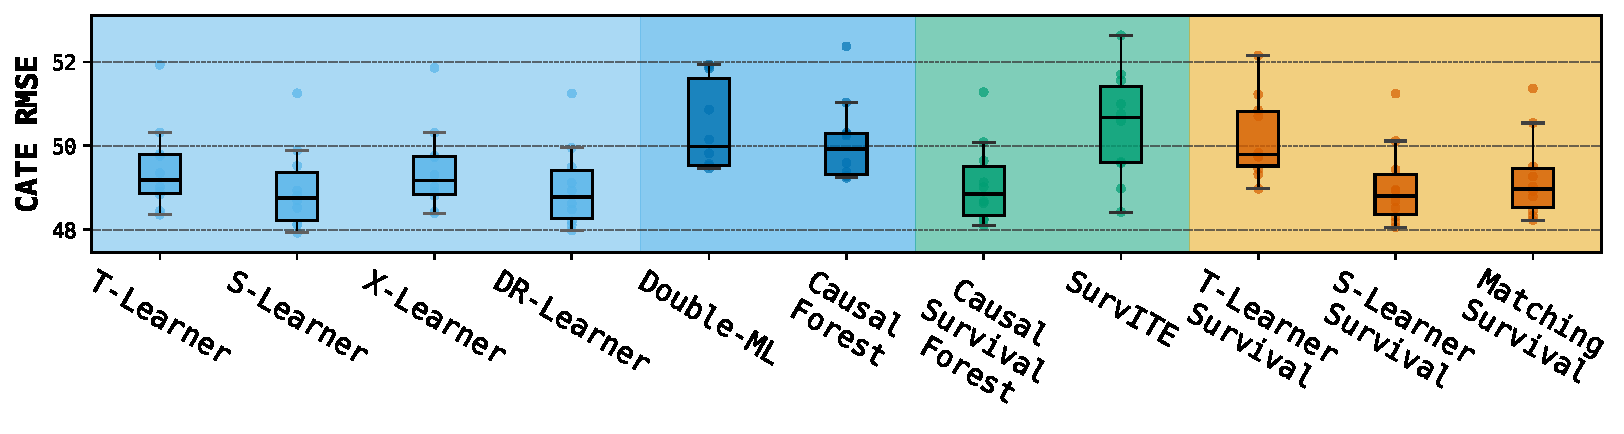
\includegraphics[width=0.7\linewidth]{Appendices/appendix-ch04/images/figure_results_updated/real_data/twin_scenario_1_twin180_cate_rmse.pdf}
   
}
\end{figure}




\subsubsection{ACTG 175 HIV clinical trial dataset} \label{ch04:subapp:hiv-data-additional-result}

We use data from the AIDS Clinical Trials Group Protocol 175 (ACTG 175) \citep{hammer1996atrial}, a double-blind, randomized controlled trial that compared four treatment regimens in adults infected with HIV type I: monotherapy with zidovudine (ZDV), monotherapy with didanosine (ddI), combination therapy with ZDV and ddI, or combination therapy with ZDV and zalcitabine (Zal).
The publicly available dataset\footnote{\url{https://archive.ics.uci.edu/dataset/890/aids+clinical+trials+group+study+175}} includes 2,139 HIV-infected patients randomized into four groups with assigned treatments: ZDV, ZDV+ddI, ZDV+Zal, and ddI.
An event occurrence was defined as the first of either a decline in CD4 cell count, an event indicating AIDS progression, or death. 

Following \citet{meir2025heterogeneous}, after fetching raw data from the UCI Machine Learning Repository, we change the resolution from days to months and add synthetic censoring based on a Bernoulli distribution with parameter $p=0.6+0.25 \cdot Z30$, where $Z30$ is a feature that is available in the data and indicates whether a patient started taking ZDV prior to the assigned treatment, and it is not included in the covariates for CATE estimation. 
We conduct three pairwise comparisons with ZDV as the baseline treatment ($W=0$): ZDV vs. ZDV+ddI (HIV1), ZDV vs. ZDV+Zal (HIV2), and ZDV vs. ddI (HIV3).
The baseline censoring rate is less than 15\% for different treatment groups.
After applying the censoring injection procedure from \citet{meir2025heterogeneous}, increasing censoring rates to over 90\%.
For each treatment group, we establish baseline CATE estimates by running Causal Survival Forests 10 times and averaging the estimated conditional average treatment effects.
Since there are many variants of outcome imputation and survival meta-learner families due to different imputation and base learner options, for display purposes in the HIV dataset results, we use a model selection criterion based on closeness (CATE RMSE) to estimation by Causal Survival Forests.
We have looked at the results using other variants of same CATE estimator as well, and similar trends are observed.

In Section~\ref{ch04:sec:real-data}, we display the comparisons of CATE estimates between baseline and high-censoring conditions for group HIV1.
Here we display the same sets of results for HIV2 and HIV3 groups in Figure~\ref{ch04:fig:hiv2-cate-estimate-comparison}, \ref{ch04:fig:hiv3-cate-estimate-comparison}.
Consistent patterns emerge across all three treatment comparisons: Causal Survival Forests produces estimates that cluster tightly around their baseline CATE estimations on data before additional censoring injection; outcome imputation methods show higher variation in baseline estimates but more concentrated predictions under high censoring, and survival meta-learners display substantial deviations from the 45-degree line, indicating sensitivity to censoring conditions.
The consistency of these patterns across different treatment pairs reinforces the robustness of our findings regarding how different estimator families respond to increased censoring.


% !TeX root = ../../../main.tex
\begin{figure}[htbp]
\ChFourFloatContents{ch04:fig:hiv2-cate-estimate-comparison}{\caption{CATE Estimation comparison between baseline and high-censoring conditions under ZDV vs. ZDV+Zal treatments (HIV2). Each point represents an individual patient in test sets, with the dashed diagonal line indicating perfect consistency between baseline CATE estimation and that with the additional censoring injected.}}{
  \centering
  
  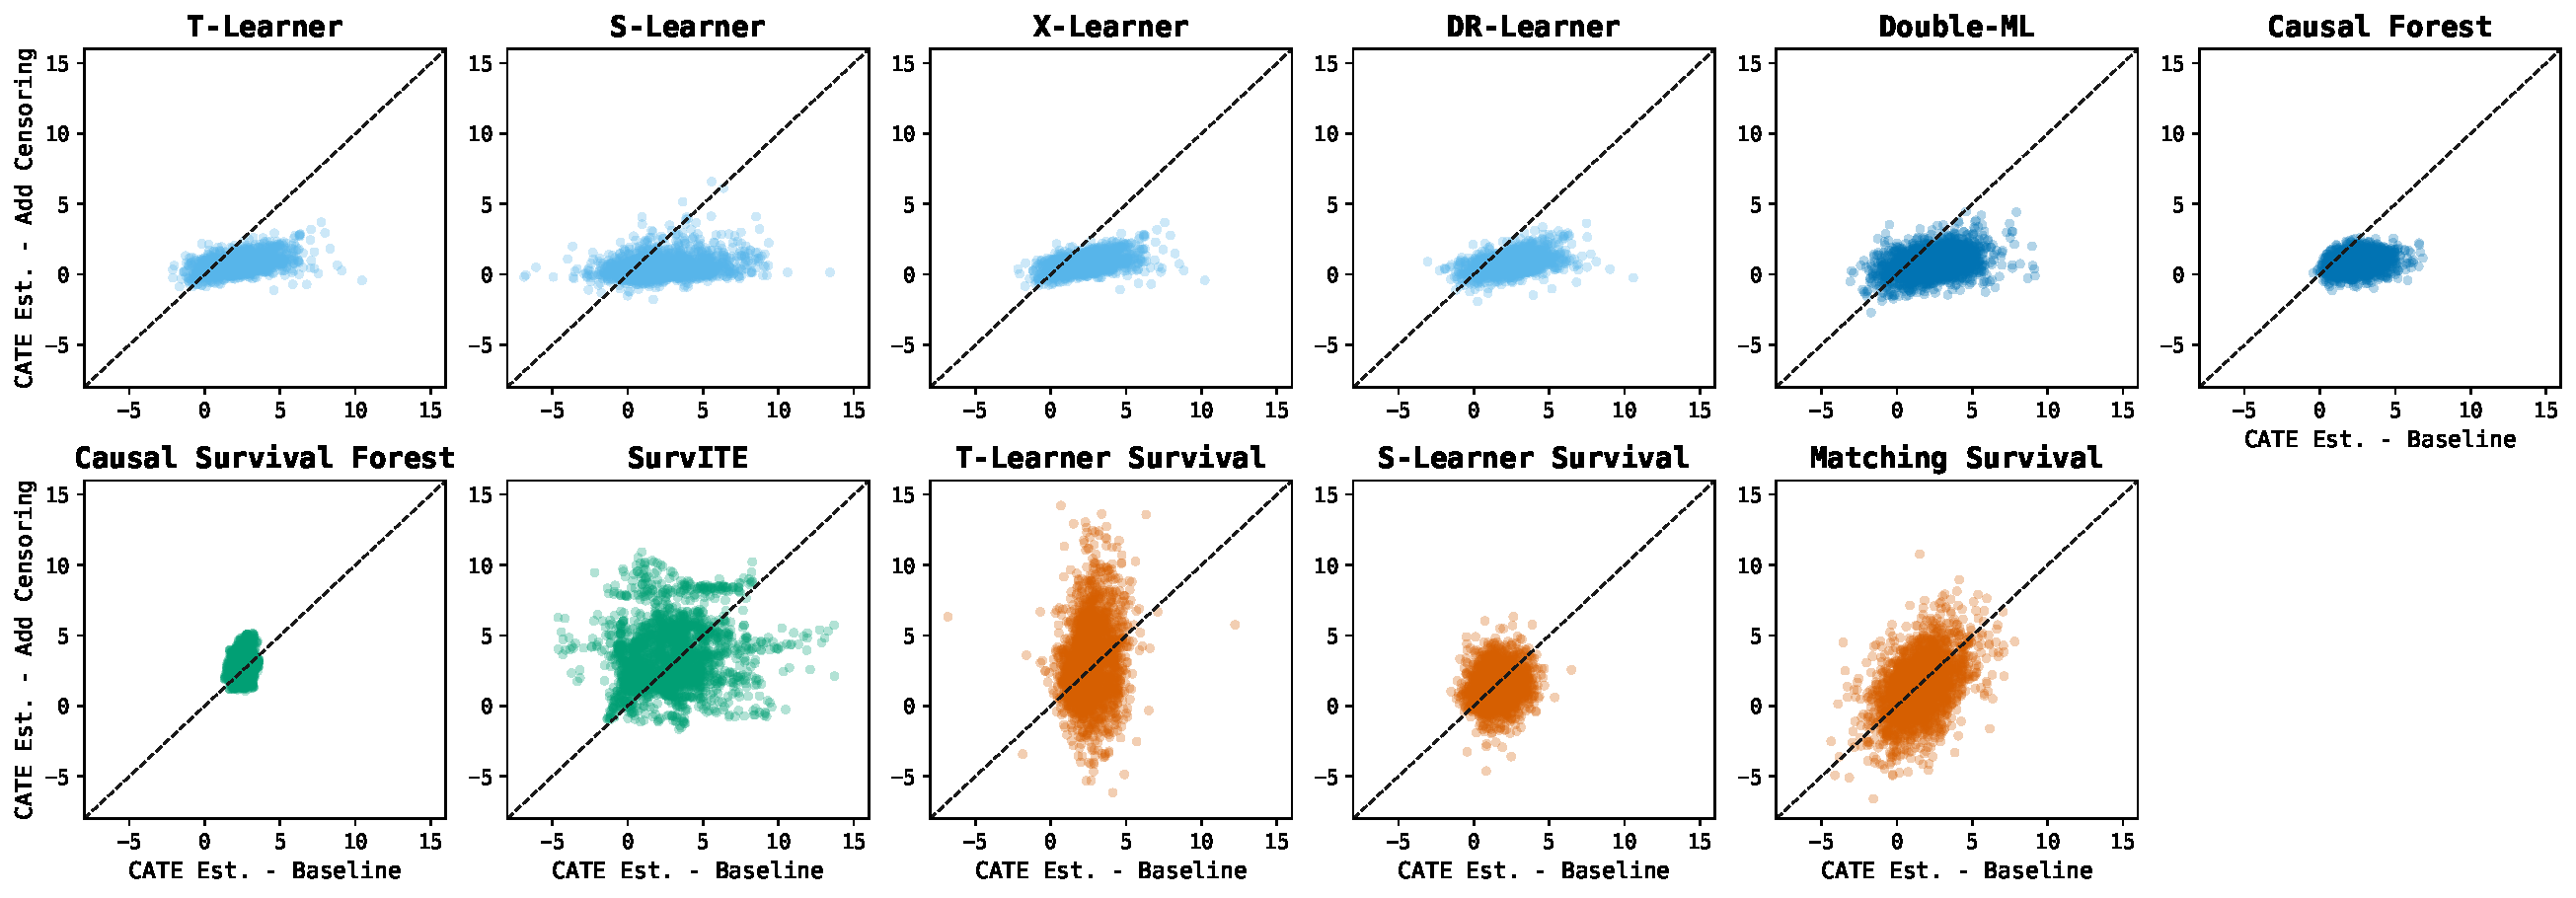
\includegraphics[width=\linewidth]{Appendices/appendix-ch04/images/figure_results_updated/real_data/ACTG_175_HIV2_CATE_comparison.pdf}
   
}
\end{figure}




% !TeX root = ../../../main.tex
\begin{figure}[htbp]
\ChFourFloatContents{ch04:fig:hiv3-cate-estimate-comparison}{\caption{CATE Estimation comparison between baseline and high-censoring conditions under ZDV vs. ddI treatments (HIV3). Each point represents an individual patient in test sets, with the dashed diagonal line indicating perfect consistency between baseline CATE estimation and that with the additional censoring injected.}}{
  \centering
  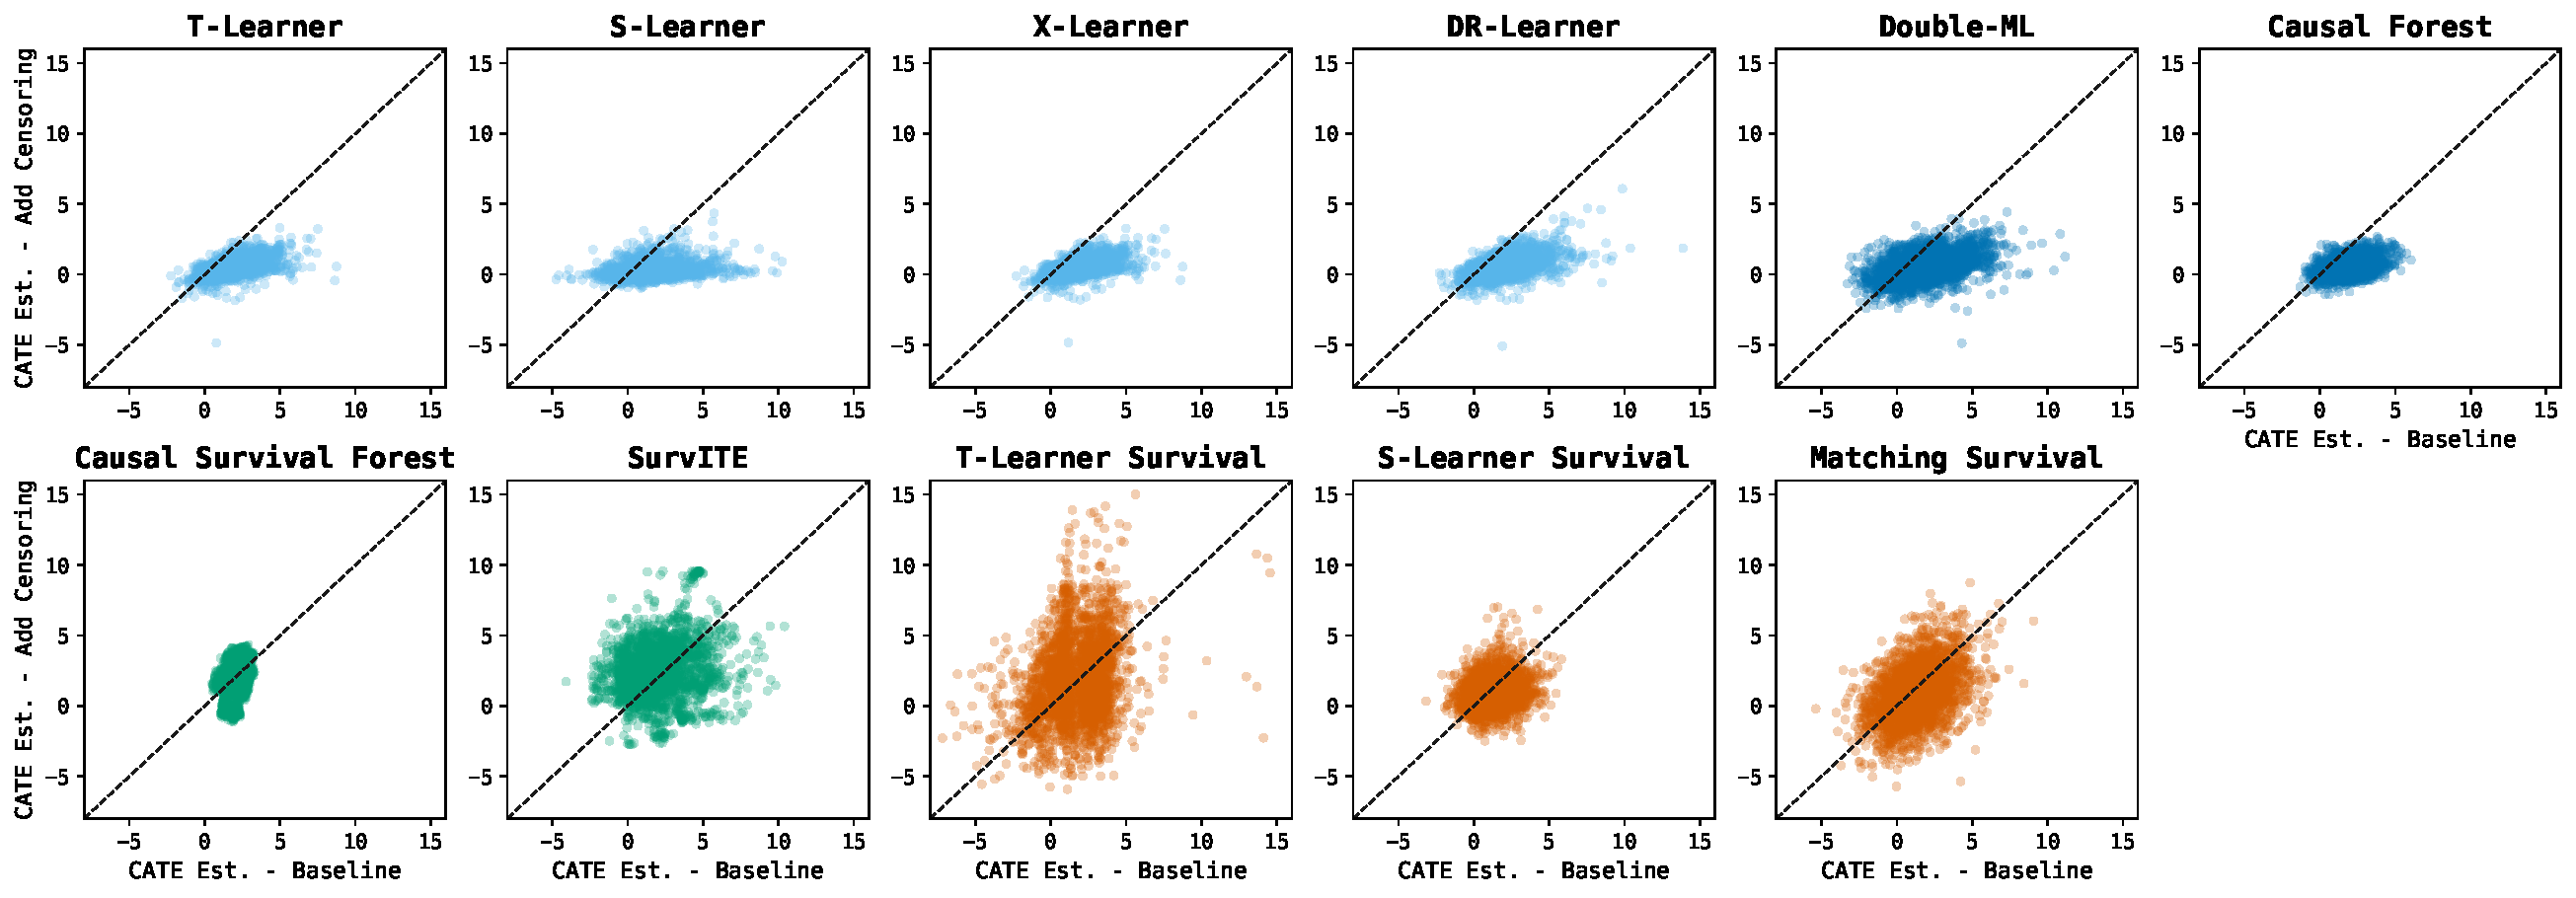
\includegraphics[width=\linewidth]
{Appendices/appendix-ch04/images/figure_results_updated/real_data/ACTG_175_HIV3_CATE_comparison.pdf}
   
}
\end{figure}






